\chapter{Implementation and Results of Dual Contouring and Dual Marching Cubes Algorithms} \label{Chapter6}

This chapter aims to provide a comprehensive overview of the implementation details and results obtained from applying the Dual Contouring (DC) and Dual Marching Cubes (DMC) algorithms for isosurface extraction. Building upon the theoretical foundations laid out in Chapter \ref{Chapter3}, the fundamental data structures introduced in Chapter \ref{Chapter4}, and the Quadratic Error Function methodology discussed in \ref{Chapter5}, this chapter will delve into the practical aspects of these algorithms. It will cover code snippets, mesh generation, and visual results, offering a holistic view of how DC and DMC can be effectively implemented and what kind of results one can expect.

\section{Dual Contouring Algorithm Overview}
In this section, we revisit the Dual Contouring algorithm, which was extensively discussed in Section \ref{Dual-Contouring}. The focus here is to lay the groundwork for the forthcoming implementation details. As a quick recap, Dual Contouring is particularly effective for preserving sharp features and handling complex topologies. 

\subsection{Implementation Steps}

The algorithm operates through a series of steps, from initializing the regular grid to solving the Quadratic Error Function for optimal point placement within grid cells. The subsequent sections will delve into the practical aspects of implementing these steps, supported by code snippets for clarity. Figure \ref{fig:dc-flow-chart} illustrates the flow diagram for the Dual Contouring algorithm. This flow diagram serves as a roadmap for the implementation, guiding the reader through the sequence of operations that transform raw data into a refined mesh. By the end of this section, the reader will clearly understand how each theoretical component from Section \ref{Dual-Contouring} translates into practical code.

\begin{figure}[H]
\centering
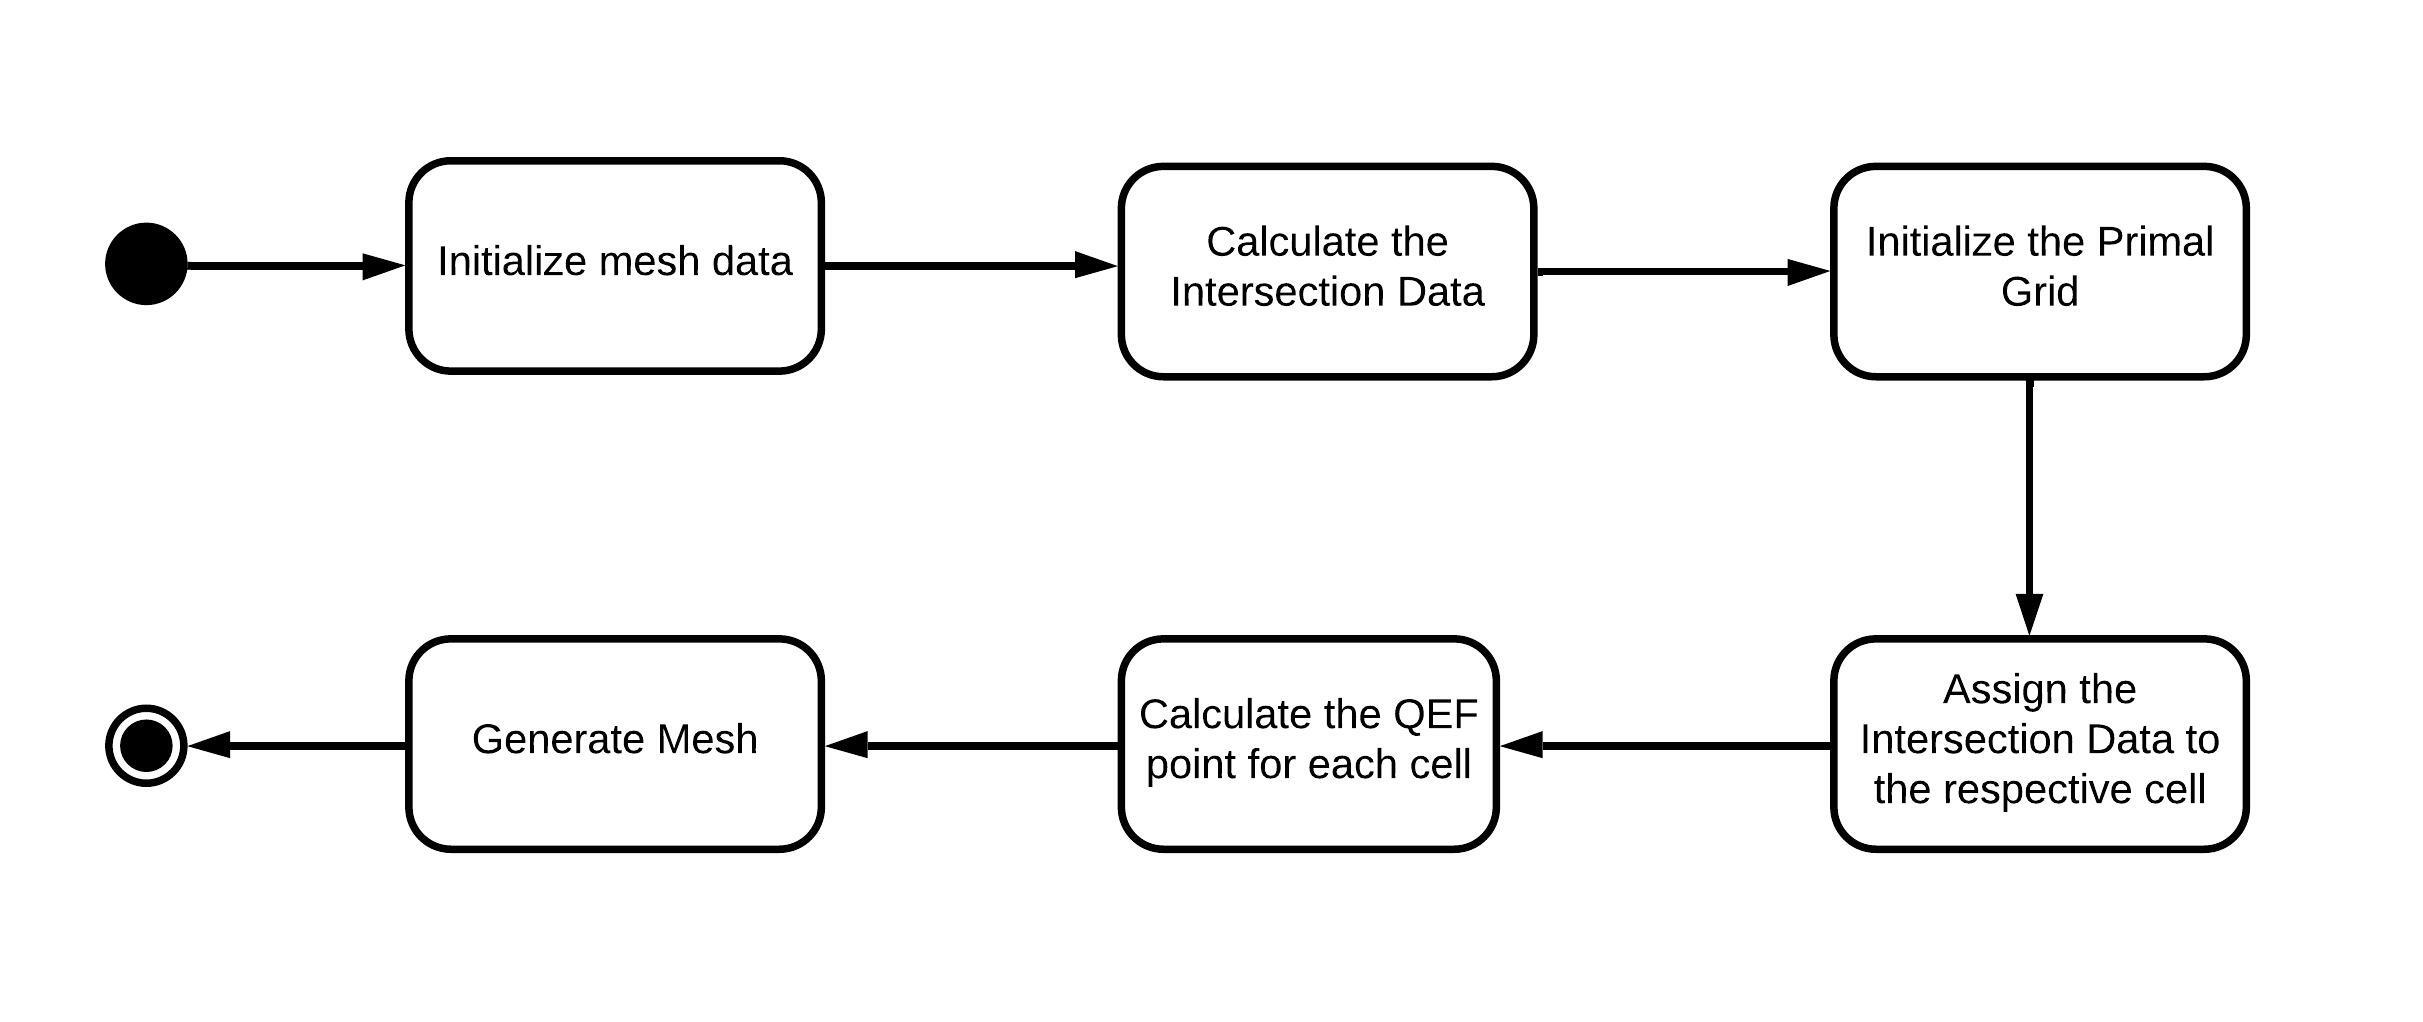
\includegraphics[width=1.0\textwidth]{Figures/DC-FlowChart.jpeg}
\decoRule
\caption{Flow chart for implementation of DC algorithm}
\label{fig:dc-flow-chart}
\end{figure}

\subsubsection{Initializing Mesh Data}

The first step in the Dual Contouring algorithm is to initialize the mesh data. This involves setting up the mesh lines along the X, Y, and Z axes. These mesh lines are crucial for firing rays in the subsequent steps and defining the primal grid where the algorithm will operate. For a more detailed explanation of what mesh lines and padded mesh lines are, refer back to Section \ref{meshLines} in Chapter \ref{Chapter4}. Here is a snippet of code (Listing \ref{lst:meshLines}) that initializes the mesh lines.

\vspace{2mm}
\begin{lstlisting}[language=C++, caption=Initializing Mesh Data, label=lst:meshLines]
std::vector<double> meshLinesX = meshData->getMeshLinesX();
std::vector<double> meshLinesY = meshData->getMeshLinesY();
std::vector<double> meshLinesZ = meshData->getMeshLinesZ();
\end{lstlisting}

The code snippet in Listing \ref{lst:meshLines} retrieves the mesh lines along the X, Y, and Z axes from a pre-populated \texttt{meshData} object. The vectors \texttt{meshLinesX}, \texttt{meshLinesY}, and \texttt{meshLinesZ} will hold the mesh lines for each respective axis. 

\subsubsection{Calculate the Intersection Data}

After initializing the mesh data, the next step is to calculate the intersection data, and for that, Intel Embree API is used. This is a crucial step for calculating and storing intersection data, which will be used later for mesh generation. The ray-casting process is detailed in Section \ref{ray-casting} of Chapter \ref{Chapter4}. Here is a snippet of code that fires rays along the mesh lines:

\begin{lstlisting}[language=C++, caption=Firing Rays Along Mesh Lines]
fireRaysAlongMeshLines(meshData);
\end{lstlisting}

The function \texttt{fireRaysAlongMeshLines} (as illustrated in Listing \ref{lst:fireRaysAlongMeshLines}) takes the pre-populated \texttt{meshData} object as an argument. This function is responsible for firing rays along the mesh lines stored in \texttt{meshData} and updating the intersection data accordingly.

\subsubsection{Initializing the Primal Grid}

The primal grid is a foundational structure in the Dual Contouring algorithm, serving as the primary framework for storing intersection data. This grid is essentially a three-dimensional structure, where each cell is an instance of the \texttt{PrimalGridCell} structure. The dimensions of this grid are determined by the sizes of the \texttt{meshLinesX}, \texttt{meshLinesY}, and \texttt{meshLinesZ} vectors, which represent the mesh lines in each respective direction.

\begin{lstlisting}[language=C++, caption=Initializing the Primal Grid, label=lst:Init-Primal-Grid]
std::vector<std::vector<std::vector<PrimalGridCell>>> primalGrid(meshLinesX.size() - 1,
    std::vector<std::vector<PrimalGridCell>>(meshLinesY.size() - 1, std::vector<PrimalGridCell>(meshLinesZ.size() - 1)));
\end{lstlisting}

The code snippet \ref{lst:Init-Primal-Grid} shows how the primal grid is initialized as a three-dimensional vector of \texttt{PrimalGridCell} structures. For a comprehensive understanding of the structure and functionality of the \texttt{PrimalGridCell} and the primal grid's significance in the context of the Dual Contouring algorithm, readers are referred to Section \ref{Data-Structures}, specifically Subsections \ref{PrimalGridCell} and \ref{Primal-Grid-Mesh} of Chapter \ref{Chapter4}.

\subsubsection{Assign Intersection Data to Respective Cell}

Once the primal grid is initialized, the next step is to populate each cell with the intersection data. This involves iterating over each cell in the grid and checking if any intersection points fall within its boundaries. If they do, these points and their corresponding normals are stored in the cell.

\begin{lstlisting}[language=C++, caption=Assigning intersection data to the primal grid cells, label=lst:sort-intersection-data]
for (int i = 0; i < meshLinesX.size() - 1; i++)
{
    for (int j = 0; j < meshLinesY.size() - 1; j++)
    {
        for (int k = 0; k < meshLinesZ.size() - 1; k++)
        {
            PrimalGridCell primalCell;

            // Define the boundaries of the current cell
            double x1 = meshLinesX[i], x2 = meshLinesX[i + 1];
            double y1 = meshLinesY[j], y2 = meshLinesY[j + 1];
            double z1 = meshLinesZ[k], z2 = meshLinesZ[k + 1];

            vector3 cellMinPoint(x1, y1, z1);
            vector3 cellMaxPoint(x2, y2, z2);

            primalCell.cellMinPoint = cellMinPoint;
            primalCell.cellMaxPoint = cellMaxPoint;

            // Check each intersection point to see if it lies within the current cell
            for (int h = 0; h < intersectionData.hitPoints.size(); h++)
            {
                vector3 hitPoint = intersectionData.hitPoints[h];
                vector3 hitNormal = intersectionData.hitNormals[h];

                if (hitPoint.isWithinBounds(cellMinPoint, cellMaxPoint, tol))
                {
                    primalCell.hitPoints.push_back(hitPoint);
                    primalCell.hitNormals.push_back(hitNormal);
                    primalCell.averagePoint += hitPoint;
                }
            }

            // If the cell contains intersection points, calculate the average and QEF point
            if (!primalCell.hitPoints.empty())
            {
                primalCell.averagePoint /= primalCell.hitPoints.size();
                primalCell.QEFPoint = calculateQEF(primalCell.hitNormals, primalCell.hitPoints, primalCell.averagePoint, primalCell.cellMinPoint, primalCell.cellMaxPoint);

            }
            else
            {
                primalCell.averagePoint = (cellMinPoint + cellMaxPoint) / 2;
            }

            primalGrid[i][j][k] = primalCell;
        }
    }
}
\end{lstlisting}

In the Listing \ref{lst:sort-intersection-data}, the nested loops iterate over each cell in the primal grid. For each cell, the boundaries are defined using the mesh lines. Then, each intersection point is checked to determine if it lies within the current cell's boundaries. If it does, the point and its corresponding normal are stored in the cell. After all intersection points have been checked for a particular cell, the average point and QEF point for the cell are calculated if the cell contains any intersection points. If the cell doesn't have any intersection points, the average point is set to the midpoint of the cell. Finally, the populated \texttt{PrimalGridCell} is assigned to its respective position in the primal grid. For a deeper understanding of the structures and functions used, readers are referred to Section \ref{Data-Structures} of Chapter \ref{Chapter4}.

\subsubsection{Calculate QEF}

The QEF is a pivotal component in the Dual Contouring algorithm, responsible for determining the optimal vertex position within a grid cell. In the previous step, the QEF was computed for cells containing intersection points using the \texttt{calculateQEF} function while assigning intersection data to each cell.

For an in-depth understanding of the QEF calculation, revisiting the comprehensive discussion in Chapter \ref{Chapter5} is recommended. In the context of this chapter, it is essential to grasp that the QEF provides a measure of error for a given vertex position within a cell. By minimizing this error, the algorithm ensures that the vertex position best represents the underlying scalar field, leading to a high-quality mesh representation.

\subsubsection{Mesh Generation}

With the intersection data assigned to the respective cells and the QEF points calculated, the last step for the Dual Contouring algorithm is to generate the mesh. This involves connecting the QEF points of adjacent cells to form the mesh triangles. Figure \ref{fig:DC-cube} provides a visual representation of this process, showcasing a cube and its corresponding mesh generated using the Dual Contouring algorithm.

\begin{figure}[H]
    \centering
    \begin{subfigure}{0.5\textwidth}
        \centering
        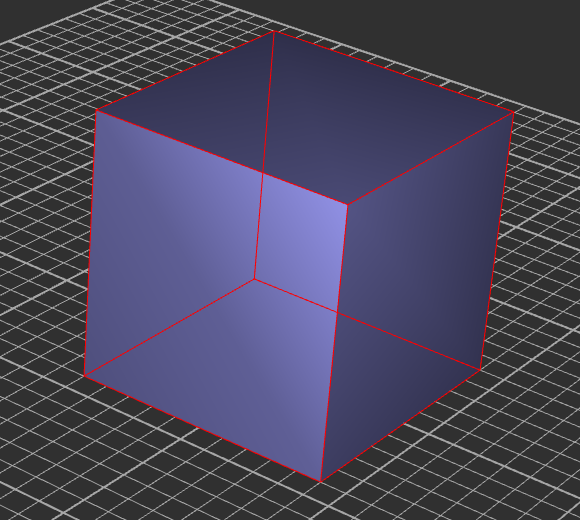
\includegraphics[height=0.7\textwidth, width=0.85\linewidth]{Figures/cube0.png}
    \end{subfigure}%
    \begin{subfigure}{0.5\textwidth}
        \centering
        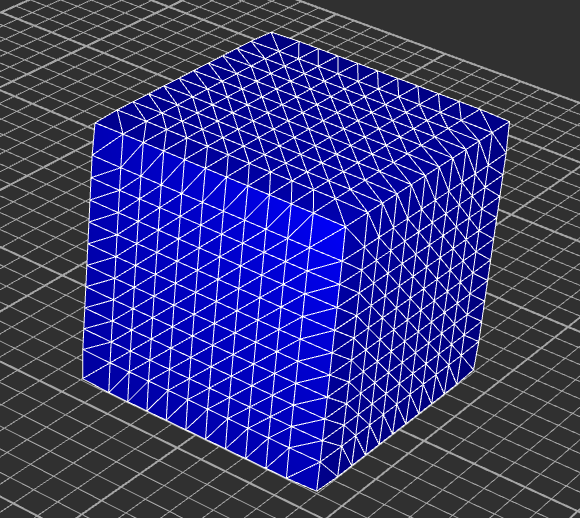
\includegraphics[height=0.7\textwidth, width=0.85\linewidth]{Figures/cube0-DC.png}
    \end{subfigure}
    \decoRule
    \caption{Cube and its mesh representation generated by the Dual Contouring algorithm.}
    \label{fig:DC-cube}
\end{figure}

In Listing \ref{lst:meshGeneration}, the code responsible for mesh generation is presented. For each cell in the primal grid, if the cell contains intersection points, the QEF point of the cell is connected with the QEF points of its adjacent cells in the positive x, y, and z directions. This algorithmic approach forms the triangles of the mesh, ensuring a coherent and accurate representation of the surface.

\vspace{2mm}
\begin{lstlisting}[language=C++, caption=Mesh Generation Using QEF Points, label=lst:meshGeneration]
for (int i = 0; i < meshLinesX.size() - 1; i++)
{
	for (int j = 0; j < meshLinesY.size() - 1; j++)
	{
		for (int k = 0; k < meshLinesZ.size() - 1; k++)
		{
			PrimalGridCell& cell = primalGrid[i][j][k];

			if (!cell.hitPoints.empty())
			{
				vector3& QEFPoint = cell.QEFPoint;

				// Connect to the cell in positive x direction
				if (i + 1 < meshLinesX.size() - 1 &&
					j + 1 < meshLinesY.size() - 1 &&
					!primalGrid[i + 1][j][k].hitPoints.empty() &&
					!primalGrid[i + 1][j + 1][k].hitPoints.empty() &&
					!primalGrid[i][j + 1][k].hitPoints.empty())
				{
					vector3& adjacentCentroidX = primalGrid[i + 1][j][k].QEFPoint;
					vector3& adjacentCentroidY = primalGrid[i][j + 1][k].QEFPoint;
					vector3& adjacentCentroidXY = primalGrid[i + 1][j + 1][k].QEFPoint;

					annotationTikhonovRegularization->addTriangle(QEFPoint.getX(), QEFPoint.getY(), QEFPoint.getZ(),
						adjacentCentroidX.getX(), adjacentCentroidX.getY(), adjacentCentroidX.getZ(),
						adjacentCentroidXY.getX(), adjacentCentroidXY.getY(), adjacentCentroidXY.getZ(), 0.0, 0.0, 0.6);

					annotationTikhonovRegularization->addTriangle(QEFPoint.getX(), QEFPoint.getY(), QEFPoint.getZ(),
						adjacentCentroidY.getX(), adjacentCentroidY.getY(), adjacentCentroidY.getZ(),
						adjacentCentroidXY.getX(), adjacentCentroidXY.getY(), adjacentCentroidXY.getZ(), 0.0, 0.0, 0.6);
				}

				// Connect to the cell in positive y direction
				if (j + 1 < meshLinesY.size() - 1 &&
					k + 1 < meshLinesZ.size() - 1 &&
					!primalGrid[i][j + 1][k].hitPoints.empty() &&
					!primalGrid[i][j][k + 1].hitPoints.empty() &&
					!primalGrid[i][j + 1][k + 1].hitPoints.empty())
				{
					vector3& adjacentCentroidY = primalGrid[i][j + 1][k].QEFPoint;
					vector3& adjacentCentroidZ = primalGrid[i][j][k + 1].QEFPoint;
					vector3& adjacentCentroidYZ = primalGrid[i][j + 1][k + 1].QEFPoint;

					annotationTikhonovRegularization->addTriangle(QEFPoint.getX(), QEFPoint.getY(), QEFPoint.getZ(),
						adjacentCentroidY.getX(), adjacentCentroidY.getY(), adjacentCentroidY.getZ(),
						adjacentCentroidYZ.getX(), adjacentCentroidYZ.getY(), adjacentCentroidYZ.getZ(), 0.0, 0.0, 0.6);

					annotationTikhonovRegularization->addTriangle(QEFPoint.getX(), QEFPoint.getY(), QEFPoint.getZ(),
						adjacentCentroidZ.getX(), adjacentCentroidZ.getY(), adjacentCentroidZ.getZ(),
						adjacentCentroidYZ.getX(), adjacentCentroidYZ.getY(), adjacentCentroidYZ.getZ(), 0.0, 0.0, 0.6);
				}

				// Connect to the cell in positive z direction
				if (k + 1 < meshLinesZ.size() - 1 &&
					i + 1 < meshLinesX.size() - 1 &&
					!primalGrid[i][j][k + 1].hitPoints.empty() &&
					!primalGrid[i + 1][j][k].hitPoints.empty() &&
					!primalGrid[i + 1][j][k + 1].hitPoints.empty())
				{
					vector3& adjacentCentroidZ = primalGrid[i][j][k + 1].QEFPoint;
					vector3& adjacentCentroidX = primalGrid[i + 1][j][k].QEFPoint;
					vector3& adjacentCentroidXZ = primalGrid[i + 1][j][k + 1].QEFPoint;

					annotationTikhonovRegularization->addTriangle(QEFPoint.getX(), QEFPoint.getY(), QEFPoint.getZ(),
						adjacentCentroidZ.getX(), adjacentCentroidZ.getY(), adjacentCentroidZ.getZ(),
						adjacentCentroidXZ.getX(), adjacentCentroidXZ.getY(), adjacentCentroidXZ.getZ(), 0.0, 0.0, 0.6);

					annotationTikhonovRegularization->addTriangle(QEFPoint.getX(), QEFPoint.getY(), QEFPoint.getZ(),
						adjacentCentroidX.getX(), adjacentCentroidX.getY(), adjacentCentroidX.getZ(),
						adjacentCentroidXZ.getX(), adjacentCentroidXZ.getY(), adjacentCentroidXZ.getZ(), 0.0, 0.0, 0.6);
				}
			}
		}
	}
}
\end{lstlisting}
\vspace{2mm}

In the mesh generation process, while the ideal representation for connecting the QEF points would be quads, due to technical constraints, triangles are used instead. When converting a quadrilateral into triangles, there are multiple ways to split it. In this implementation, the QEF point of a cell is connected with the QEF points of its adjacent cells in the positive x, y, and z directions. For each connection direction, two triangles are formed to represent the surface of the quadrilateral. For instance, when connecting in the positive x direction, one triangle is formed using the QEF point, the adjacent QEF point in the x direction, and the QEF point in the combined x-y direction. A second triangle is then formed using the QEF point, the adjacent QEF point in the y direction, and the QEF point in the combined x-y direction. This methodical approach ensures that the resulting triangles accurately represent the underlying surface and maintain the integrity of the mesh.

\section{Dual Marching Cubes Implementation} \label{sec:dmc-implementation}

In this section, we revisit the Dual Marching Cubes algorithm, comprehensively explored in Section \ref{Dual-Marching-Cubes} of Chapter \ref{Chapter3}. The primary focus here is to bridge the gap between the theoretical underpinnings and the practical implementation of the algorithm. To briefly recap, the Dual Marching Cubes algorithm is renowned for generating adaptive, topologically accurate meshes that faithfully reproduce thin features, marking it as a significant advancement in isosurface extraction.

\subsection{Algorithm Overview}

The Dual Marching Cubes algorithm builds upon the robustness of Marching Cubes and the adaptability of Dual Contouring, aiming to produce detailed and topologically sound meshes. It operates through a sequence of steps, from constructing a dual grid to refining the generated mesh using Quadratic Error Function calculations. The following sections provide a detailed walkthrough of these steps, accompanied by code snippets for a clearer understanding. Figure \ref{fig:dmc-flow-chart} presents a flow diagram to guide the reader through the DMC algorithm's implementation process. This diagram serves as a roadmap, elucidating how each theoretical concept from Section \ref{Dual-Marching-Cubes} is translated into actionable code.

While sharing some similarities with Dual Contouring, the Dual Marching Cubes algorithm introduces unique steps that focus on the dual grid of the scalar field. This section provides a detailed walkthrough of the DMC implementation, divided into three main parts.

\begin{figure}[ht!]
\centering
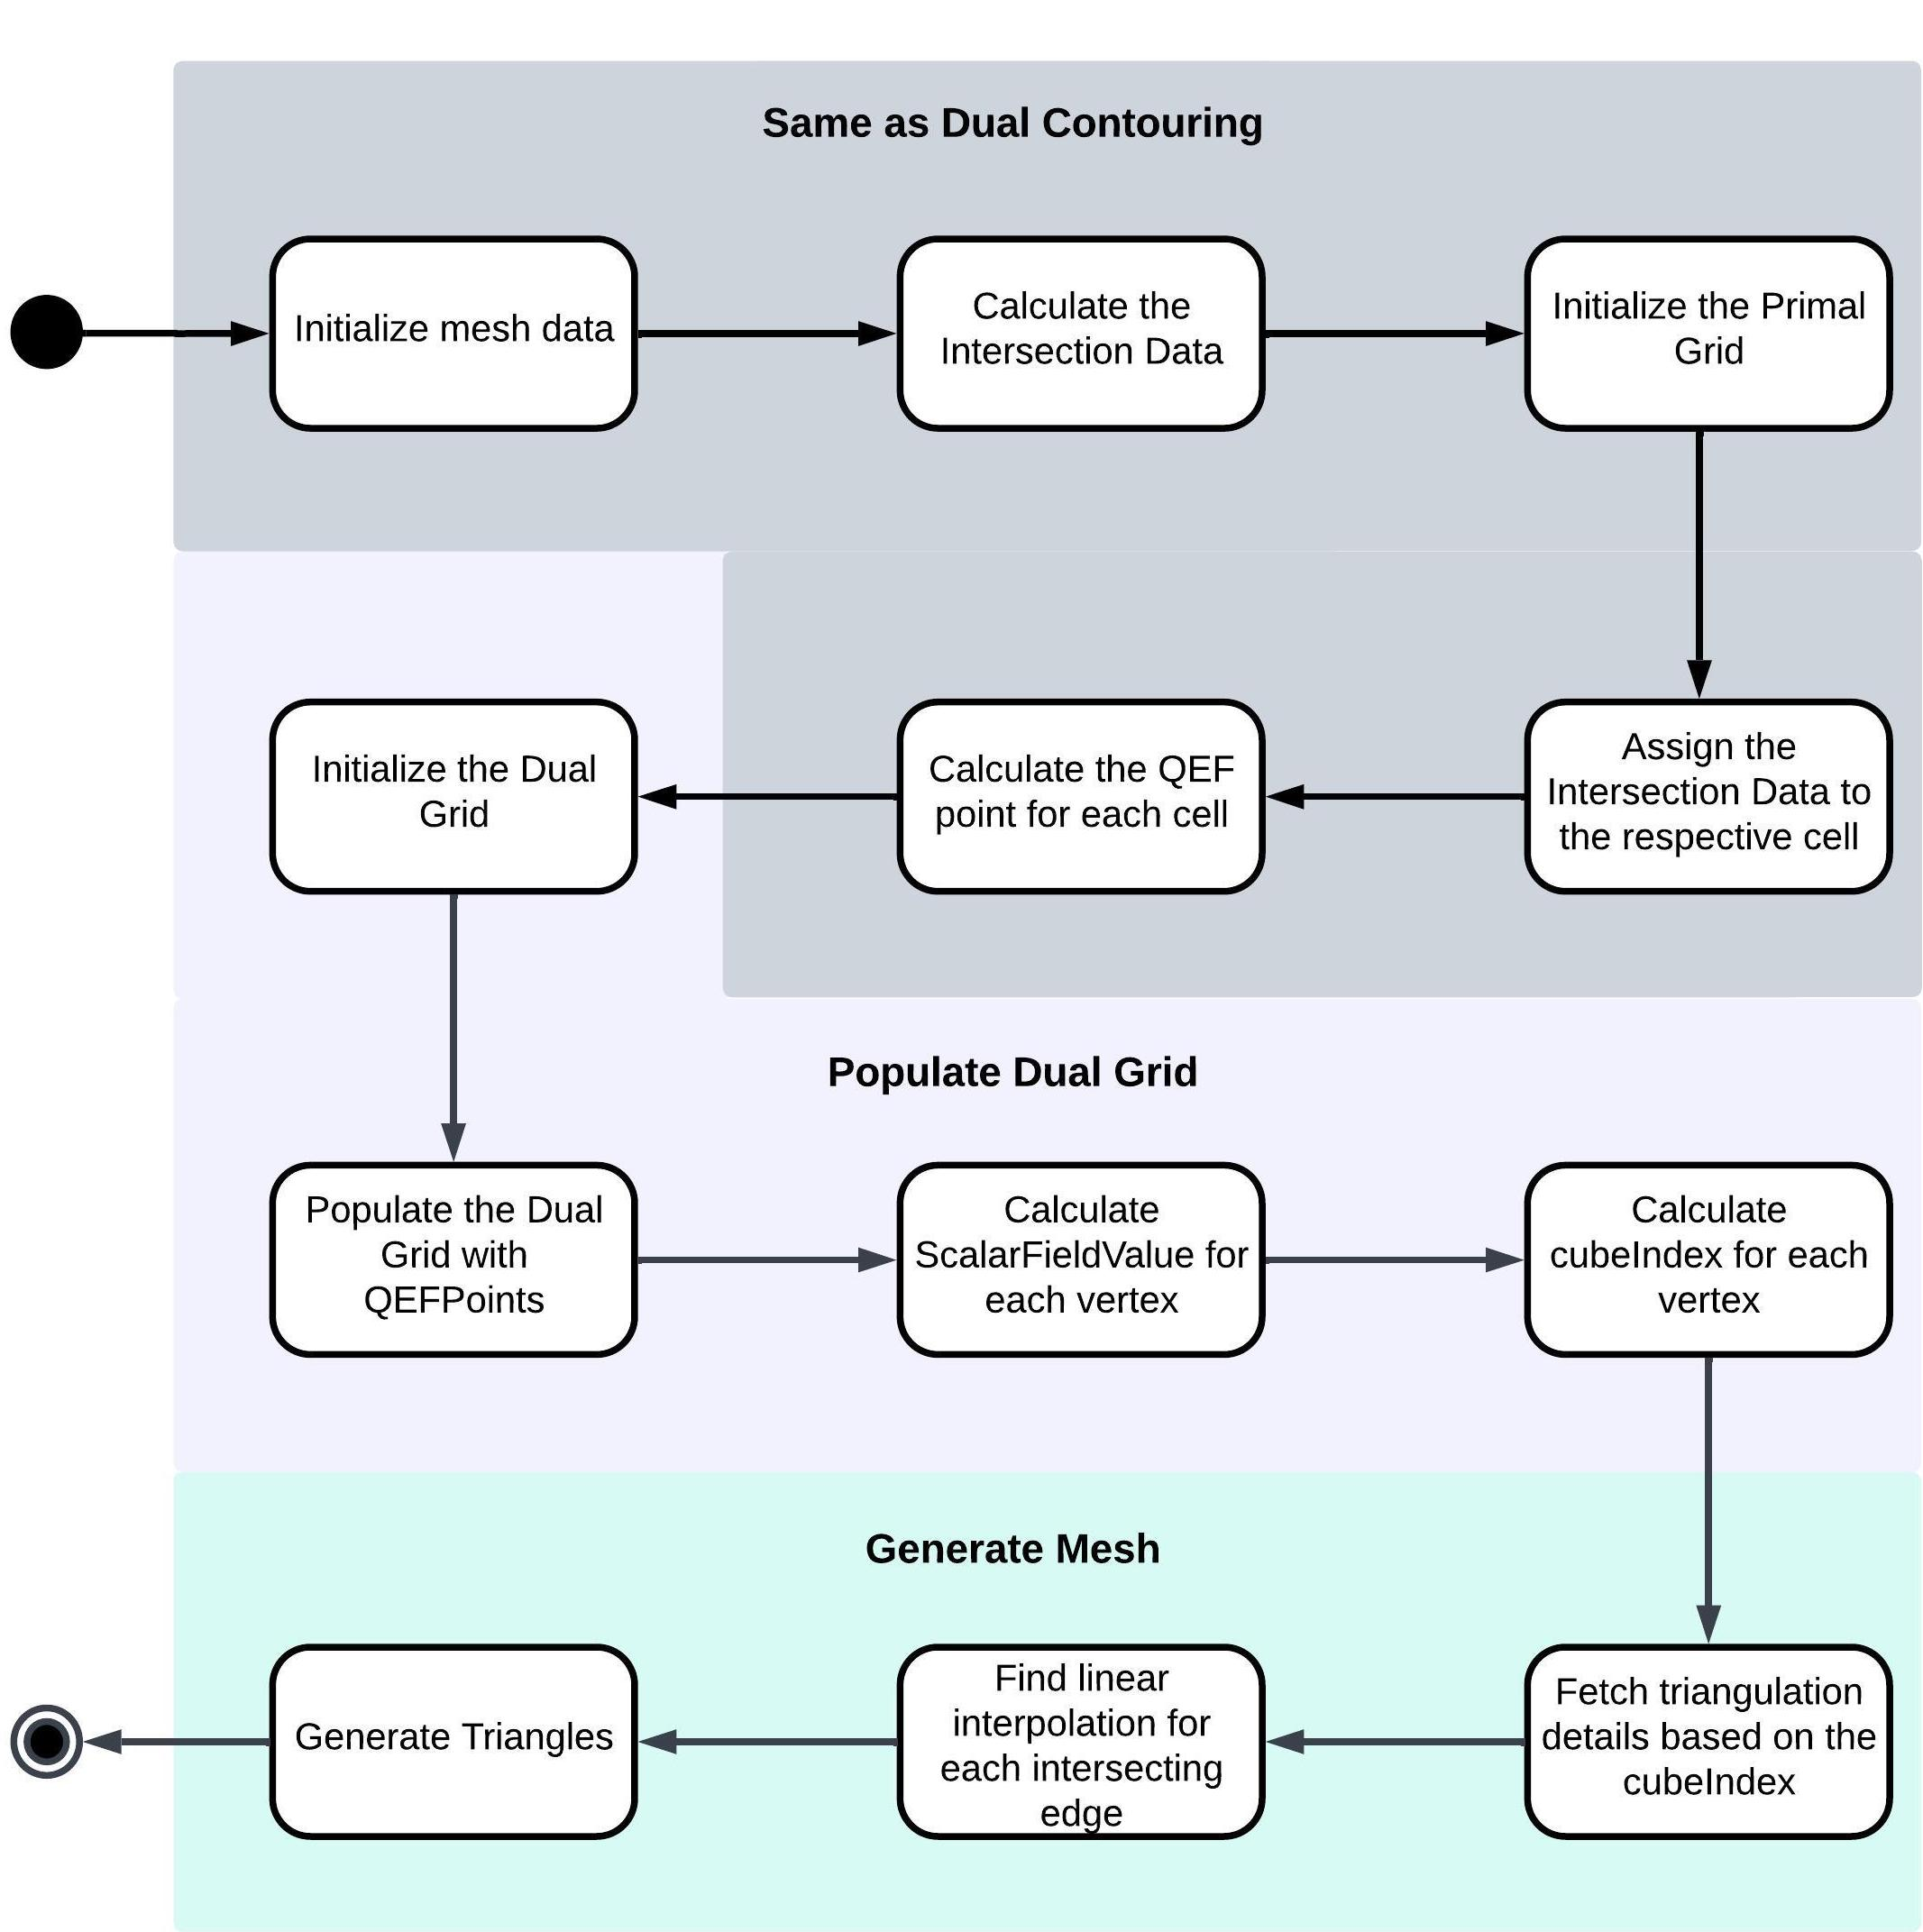
\includegraphics[width=1.0\textwidth]{Figures/DMC-FlowChart.jpeg}
\decoRule
\caption{Flow chart for implementation of DMC algorithm}
\label{fig:dmc-flow-chart}
\end{figure}

\subsection{Shared Foundations with Dual Contouring}

The initial steps of the DMC algorithm mirror those of Dual Contouring. This phase ensures that the foundational data structures and initial computations are in place, setting the stage for the unique aspects of DMC.

% Here, you can briefly mention the steps that are the same as in DC without going into the details since they were covered in the previous section.

\subsection{Populating the Dual Grid} \label{populating-dual-grid}

As the name suggests, the Dual Marching Cubes algorithm introduces a dual grid structure that complements the primal grid used in the initial stages. This dual grid is pivotal in the algorithm's ability to generate topologically accurate and feature-preserving meshes. Populating this grid is a multi-faceted process that ensures the grid is equipped with all the necessary data points and attributes required for the subsequent mesh generation phase.

This section will delve into the intricacies of initializing and populating the dual grid. This involves setting up the grid's structure, assigning values, determining scalar field values for each vertex, and calculating the cube index that will guide the triangulation process. Each of these steps is crucial in ensuring that the dual grid is primed for the final mesh generation, and we will explore them in detail in the following subsections.

\subsubsection{Initialization of the Dual Grid}

The initialization of the dual grid is a foundational step in the Dual Marching Cubes algorithm. This grid, constructed using a nested vector list, serves as the primary data structure that will hold the vertices, scalar field values, and other essential attributes required for the subsequent algorithm steps.

\vspace{2mm}
\begin{lstlisting}[language=C++, caption=Initializing the Dual Grid, label=lst:dualGridInit]
std::vector<std::vector<std::vector<DualGridCell>>> dualGrid(
    paddedMeshLinesX.size() - 1,
    std::vector<std::vector<DualGridCell>>(
        paddedMeshLinesY.size() - 1,
        std::vector<DualGridCell>(paddedMeshLinesZ.size() - 1)
    )
);
\end{lstlisting}
The code snippet in Listing \ref{lst:dualGridInit} initializes the dual grid using a 3D nested vector list. Each cell in this grid corresponds to the \texttt{DualGridCell} structure, as detailed in Section \ref{DualGridCell}. The grid's dimensions are defined by the \texttt{paddedMeshLines} across the X, Y, and Z axes, which, as mentioned in Section \ref{meshLines}, are enhanced mesh lines tailored for efficient boundary handling. This nested vector representation, highlighted in Section \ref{Dual-Grid-Mesh}, not only ensures efficient data storage and quick access but also simplifies the implementation process. Such a structure is crucial for the Dual Marching Cubes algorithm, offering a robust framework for mesh generation data processing.

\subsubsection{Populating the Dual Grid with QEF Points}
Once the dual grid is initialized, the next crucial step is to populate it with the QEF points. These points are derived from the primal grid and represent the optimal vertex positions within each cell of the dual grid.

\vspace{2mm}
\begin{lstlisting}[language=C++, caption=Populating the Dual Grid with QEF Points, label=lst:populateDualGrid]
double isovalue = 0.5;
for (int i = 0; i < paddedMeshLinesX.size() - 2; i++) {
    for (int j = 0; j < paddedMeshLinesY.size() - 2; j++) {
        for (int k = 0; k < paddedMeshLinesZ.size() - 2; k++) {
            DualGridCell& dualCell = dualGrid[i][j][k];  
    
            dualCell.vertices[0] = getVertexFromPaddedPrimalCell(i, j, k, paddedPrimalGrid);
            dualCell.vertices[1] = getVertexFromPaddedPrimalCell(i + 1, j, k, paddedPrimalGrid);
            dualCell.vertices[2] = getVertexFromPaddedPrimalCell(i + 1, j + 1, k, paddedPrimalGrid);
            dualCell.vertices[3] = getVertexFromPaddedPrimalCell(i, j + 1, k, paddedPrimalGrid);
            dualCell.vertices[4] = getVertexFromPaddedPrimalCell(i, j, k + 1, paddedPrimalGrid);
            dualCell.vertices[5] = getVertexFromPaddedPrimalCell(i + 1, j, k + 1, paddedPrimalGrid);
            dualCell.vertices[6] = getVertexFromPaddedPrimalCell(i + 1, j + 1, k + 1, paddedPrimalGrid);
            dualCell.vertices[7] = getVertexFromPaddedPrimalCell(i, j + 1, k + 1, paddedPrimalGrid);
    
            //Populate scalar field values
            for (int v = 0; v < 8; v++) {
                const vector3& vertex = dualCell.vertices[v];
                bool inside = testPointInside(vertex.getX(), vertex.getY(), vertex.getZ());
                dualCell.scalarFieldValues[v] = inside ? 1.0 : 0.0;  
    
                if (dualCell.scalarFieldValues[v] > isovalue) {
                    dualCell.cubeIndex |= 1 << v;
                }
            }
        }
    }
}
\end{lstlisting}
\vspace{2mm}

The dual grid vertices are constructed by iterating through the padded mesh lines in the above code snippet (Listing \ref{lst:populateDualGrid}). For each cell in the dual grid, the vertices are populated using the \texttt{getVertexFromPaddedPrimalCell} function, which fetches the QEF point (or centroid) from the corresponding cell in the padded primal grid.

\vspace{2mm}
\begin{lstlisting}[language=C++, caption=Fetching Vertex from Padded Primal Cell, label=lst:getVertex]
Vector3 getVertexFromPaddedPrimalCell(int i, int j, int k, const std::vector<std::vector<std::vector<PrimalGridCell>>>& paddedPrimalGrid) {
	// If coordinates are out of bounds, return an empty vector
	if (i >= paddedPrimalGrid.size() || j >= paddedPrimalGrid[0].size() || k >= paddedPrimalGrid[0][0].size()) {
		return vector3::Empty();
	}

	const PrimalGridCell& primalCell = paddedPrimalGrid[i][j][k];

	// Check if QEFPoint is set (not equal to zero vector)
	if (primalCell.QEFPoint != vector3::Empty()) {
		return primalCell.QEFPoint;
	}
	else {
		// Compute the center of the PrimalGridCell
		return (primalCell.cellMinPoint + primalCell.cellMaxPoint) / 2.0;
	}
}
\end{lstlisting}
\vspace{2mm}

The function \texttt{getVertexFromPaddedPrimalCell} (Listing \ref{lst:getVertex}) checks if the QEFPoint for the corresponding primal cell is set. If it is, this point is returned. Otherwise, the function computes and returns the center of the primal cell. This process ensures that the dual grid is populated with optimal vertex positions, setting the stage for the subsequent steps in the Dual Marching Cubes algorithm.

\subsubsection{Calculating Scalar Field Values for Each Vertex}

After populating the dual grid with QEF points, the next step is to compute the scalar field values for each vertex of the dual grid. These scalar field values are essential for determining the topology of the isosurface within each cell.

In the code snippet from Listing \ref{lst:populateDualGrid}, the scalar field values are determined based on whether a vertex is inside or outside the isosurface. A simple test function, \texttt{testPointInside}, is used to check the position of the vertex relative to the isosurface. If the vertex is inside, it is assigned a scalar field value of \(1.0\); otherwise, it is given a value of \(0.0\).

\subsubsection{Determining the Cube Index for Each Vertex}

The cube index is a crucial component in the Dual Marching Cubes algorithm. It represents the configuration of the cell based on the scalar field values of its vertices and determines how the cell will be triangulated.

In the same code snippet (Listing \ref{lst:populateDualGrid}), the cube index for each dual grid cell is computed after populating the scalar field values. This is done by iterating the scalar field values of the cell's vertices and comparing them to a predefined isovalue (set to \(0.5\) in the code). If the scalar field value of a vertex is greater than the isovalue, the corresponding bit in the cube index is set. This cube index will later fetch the appropriate triangulation details from the Marching Cubes lookup table, facilitating the mesh generation process.

\subsection{Mesh Generation}

The mesh generation phase in the Dual Marching Cubes algorithm is pivotal. It translates the populated dual grid into a coherent mesh representation. This process involves fetching the triangulation details for each cell based on its cube index, determining the intersection points on the edges, and finally generating the triangles that form the mesh.

\subsubsection{Fetching Triangulation Details}

The triangulation details for each cell are fetched from a predefined lookup table called the triangulation table. This table contains the triangulation patterns for all 256 possible cell configurations. The cell's cube index, computed earlier, serves as the key to fetch the appropriate triangulation pattern. The edge table and triangulation table provided in Listing \ref{lst:triangulationTable} are essential components for this process.

\vspace{2mm}
\begin{lstlisting}[language=C++, caption=Edge and Triangulation Tables, label=lst:triangulationTable]
// This is the edge table
std::vector<std::pair<int, int>> edges = {
	{0, 1}, {1, 2}, {2, 3}, {3, 0},  // Bottom face
	{4, 5}, {5, 6}, {6, 7}, {7, 4},  // Top face
	{0, 4}, {1, 5}, {2, 6}, {3, 7}   // Connecting lines
};

// This is the triangulation table
std::vector<std::vector<std::vector<int>>> triangulationTable = {
	{},
	{{8, 0, 3}},
	// ... all 256 cases
	{{3, 0, 8}},
	{}
};
\end{lstlisting}

\subsubsection{Linear Interpolation for Intersecting Edges}

The algorithm (Listing \ref{lst:meshGenerationDMC}) first fetches the triangulation pattern from the triangulation table for each cell in the dual grid. Once the triangulation pattern is identified, the edges that form these triangles are determined. These edges are crucial as they potentially intersect the isosurface.

To find the exact intersection points on these edges, the algorithm fires a ray (Listing \ref{lst:castRay}) from one vertex of the edge to the other, leaving a small offset on both sides. This ray-tracing approach, facilitated by the Embree API, precisely determines where the edge intersects the isosurface. As soon as the ray intersects with the surface, the interpolation details are captured, providing the exact position of the intersection point.

Ensuring that the intersection point genuinely lies on the edge segment between the two vertices is essential. For this purpose, the \texttt{isOnSegment} function is employed (Listing \ref{lst:isOnSegment}). This function checks the collinearity of three points: the two vertices of the edge and the intersection point. It is considered valid if the intersection point is collinear and lies between the two vertices. As described earlier, the \texttt{isOnSegment} function uses both the dot product and cross product to verify the collinearity and position of the intersection point relative to the edge segment.

This combined approach of ray tracing and segment validation ensures that the generated triangles accurately represent the underlying scalar field and are free from artifacts or inaccuracies.

\vspace{2mm}
\begin{lstlisting}[language=C++, caption=Mesh generation in Dual Marching Cubes Algorithm, label=lst:meshGenerationDMC]
for (int i = 0; i < dualGrid.size(); i++)
{
	for (int j = 0; j < dualGrid[0].size(); j++)
	{
		for (int k = 0; k < dualGrid[0][0].size(); k++)
		{
			DualGridCell dualCell = dualGrid[i][j][k];

			// Get the triangulation pattern for the current cell
			std::vector<std::vector<int>> triangulationPattern = triangulationTable[dualCell.cubeIndex];

			// Iterate over each triangle in the triangulation pattern
			for (const auto& triangle : triangulationPattern) 
			{
				// Clear previous intersection data
				intersectionData.hitPoints.clear();
				intersectionData.hitNormals.clear();

				std::vector<vector3> triangleIntersectionPoints;

				// Iterate over each edge in the triangle
				for (int t : triangle) 
				{
					// Extract the vertices of the current edge
					const auto& edge = edges[t];
					const vector3& vertex1 = dualCell.vertices[edge.first];
					const vector3& vertex2 = dualCell.vertices[edge.second];
					
					// Compute the direction and normalized direction of the edge
					vector3 dir = vertex2 - vertex1;
					float dirLength = dir.length();
					vector3 normalizedDir = dir / dirLength;

					// Offset for avoiding precision issues
					vector3 offset = normalizedDir * 1e-2f;
					vector3 start = vertex1 - offset;
					vector3 end = vertex2 + offset;

					// Cast a ray from the start in the direction of the edge
					castRay(scene, start.getX(), start.getY(), start.getZ(), dir.getX(), dir.getY(), dir.getZ());

					// If there are intersection points
					if (!intersectionData.hitPoints.empty())
					{
						bool flag = false;
						// If there's more than one intersection point
						if (!(intersectionData.hitPoints.size() == 1)) 
						{
							// Check if the intersection point lies on the segment
							for (int m = 0; m < intersectionData.hitPoints.size(); m++)
							{
								vector3 hitPoint = intersectionData.hitPoints[m];
								if(isOnSegment(start, end, hitPoint))
								{
									triangleIntersectionPoints.push_back(hitPoint);
									flag = true;
								}
							}
						}
                        else 
                        {
                        	triangleIntersectionPoints.push_back(intersectionData.hitPoints[0]);
                        }
						// Clear the intersection data for the next iteration
						intersectionData.hitPoints.clear();
						intersectionData.hitNormals.clear();
					}
				}

				// If we have at least 3 intersection points, form a triangle
				if (triangleIntersectionPoints.size() >= 3) 
				{
					annotationSVD->addTriangle(
						triangleIntersectionPoints[0].getX(), triangleIntersectionPoints[0].getY(), triangleIntersectionPoints[0].getZ(),
						triangleIntersectionPoints[1].getX(), triangleIntersectionPoints[1].getY(), triangleIntersectionPoints[1].getZ(),
						triangleIntersectionPoints[2].getX(), triangleIntersectionPoints[2].getY(), triangleIntersectionPoints[2].getZ(),
						r, g, b
					);
				}
                    else
				{
					//Less than 3 intersection points, something is wrong
					displayMessage("Triangle has less than 3 intersection points\n");
				}
			}
		}
	}
}

\end{lstlisting}

\vspace{2mm}
\begin{lstlisting}[language=C++, caption=Checking Point Collinearity, label=lst:isOnSegment]
bool isOnSegment(vector3& v1, vector3& v2,vector3& p)
{
    // Compute the vector from v1 to v2
	vector3 v1v2 = v2 - v1;
    
    // Compute the vector from v1 to p
	vector3 v1p = p - v1;

    // Compute the dot product between v1v2 and v1p
	float dotProduct = v1v2.dot(v1p);
    
    // Compute the squared length of v1v2
	float sqLength_v1v2 = v1v2.dot(v1v2);

    // check point p is in the same direction as v2 and lies in between
	if (dotProduct >= 0 && dotProduct <= sqLength_v1v2) 
    {
		// check for collinearity
		vector3 crossProduct = v1v2.cross(v1p);
        
        // Small threshold to handle floating point inaccuracies
		const float epsilon = 1e-4;
        
        // If the length of the cross product is close to zero, then v1, p, and v2 are collinear
		if (crossProduct.length() < epsilon) 
        {
			return true; // p lies on the line segment between v1 and v2
		}
	}
    
    // p does not lie on the line segment between v1 and v2
	return false;
}
\end{lstlisting}

\subsubsection{Triangle Generation}

With the intersection points on the edges identified, the subsequent phase involves constructing the triangles that will constitute the mesh. The triangulation pattern, previously fetched from the triangulation table, serves as a guide for this process. 

In the algorithm, as illustrated in Listing \ref{lst:meshGenerationDMC}, a crucial check is performed: it ensures that exactly three points are available to form a triangle. If this condition is met, the triangle is added to the mesh. However, if there aren't three points, it indicates an anomaly in the triangulation process. While such anomalies might warrant further investigation in a comprehensive study, they fall outside the scope of this thesis and are not delved into further.

\section{Results and Discussion}

The results of the Dual Contouring and Dual Marching Cubes algorithms were evaluated on various datasets, ranging from simple geometric shapes to complex real-world data. The primary focus was to assess the quality of the generated meshes, the preservation of sharp features, and the efficiency of the algorithms.

\subsection{Quality of Generated Meshes}

\subsubsection{Dual Contouring} 
The DC algorithm produced high-quality meshes, especially in datasets with sharp features. As discussed in Section \ref{Dual-Contouring}, the DC algorithm preserved sharp edges and corners, which were smoothed out by the Marching Cubes algorithm. However, the DC algorithm sometimes produced non-manifold meshes in scenarios with large flat surfaces or when multiple objects were in close proximity.
\begin{figure}[h]
    \centering
    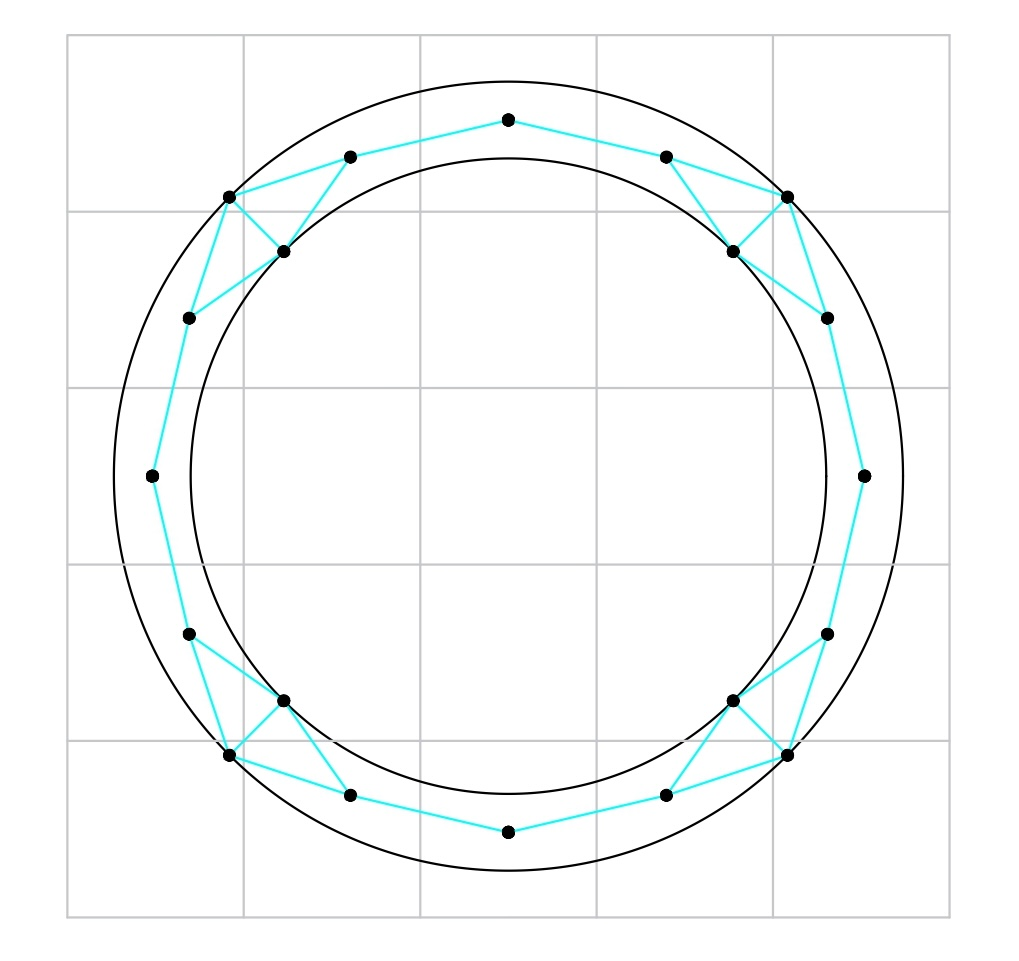
\includegraphics[width=0.52\textwidth]{Figures/DC-manifold-example.jpg}
    \decoRule
    \caption{Visualization of the Dual Contouring algorithm's limitation permits only a single vertex per cell.}
    \label{fig:DC-limitation-ch6}
\end{figure}
As illustrated in Fig. \ref{fig:DC-limitation-ch6}, the object is represented by a very thin ring in black. The QEF point is denoted by the black vertex. The cyan color highlights the surface generated using the Dual Contouring algorithm. Due to the algorithm's limitation of allowing only one vertex per cell, the ring appears infinitely thin. This representation also results in degenerated triangles, which can be observed in the cyan surface.

\subsubsection{Dual Marching Cubes} 
The Dual Marching Cubes algorithm excelled in representing thin-walled structures and intricate thin features. In Figure \ref{fig:DMC-dual-grid-ex-ch6}, a two-dimensional example is presented to elucidate the Dual Marching Cubes algorithm's workings with thin features. The primal grid, foundational to the process, is depicted in light grey. The QEF points, integral to the algorithm, are distinctly marked as black vertices. By connecting these QEF points, we form the dual grid, which is emphasized in contrasting red. The original object, a thin ring, is outlined in black. When the DMC algorithm is applied, the resultant surface, shown in cyan, emerges. Due to the mesh's granularity, the resultant surface is slightly imperfect curvature.

\begin{figure}[H]
\centering
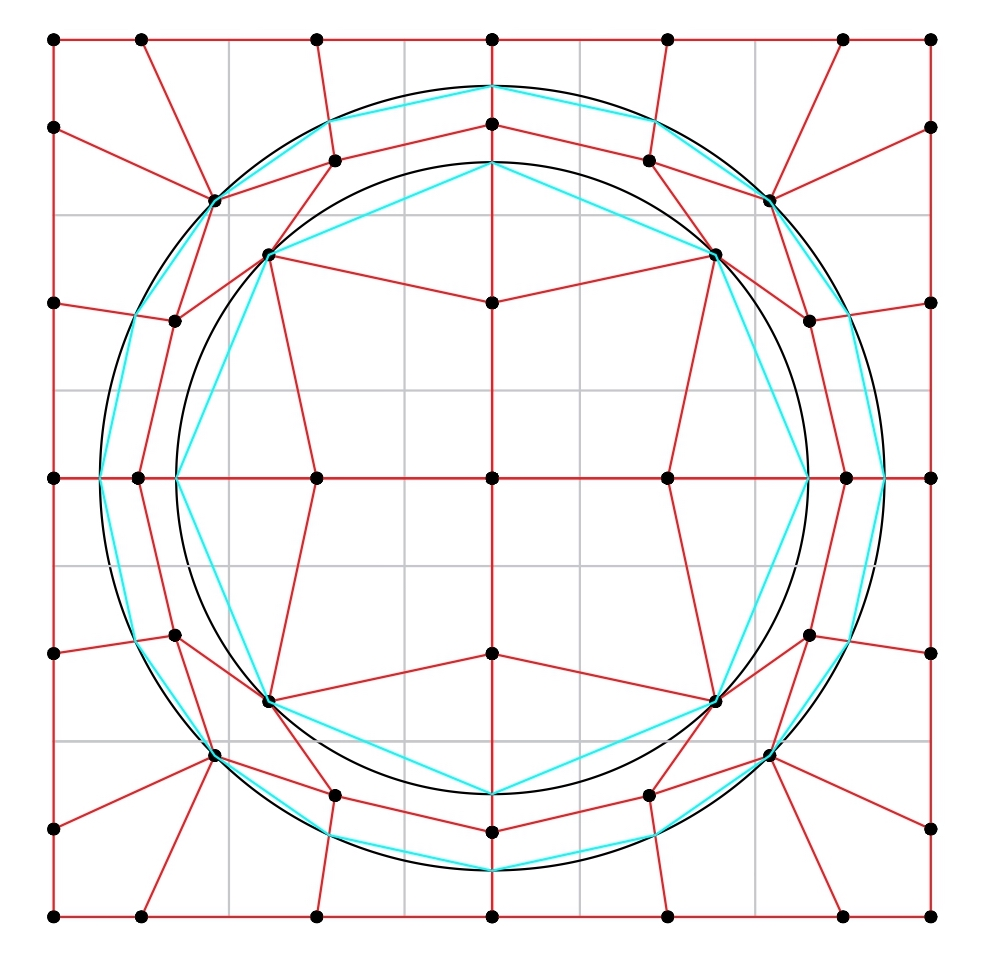
\includegraphics[width=0.5\textwidth]{Figures/DMC-dual-grid.jpg}
\decoRule
\caption{2D visualization of the Dual Marching Cubes Algorithm on a thin ring}
\label{fig:DMC-dual-grid-ex-ch6}
\end{figure}

\subsection{Advantages and Limitations in Practice}

In practical applications, the advantages and limitations of both algorithms became evident. The DC algorithm's ability to preserve sharp features was evident in datasets with geometric shapes, while its limitations (Fig. \ref{fig:DC-analysis-thin-features}), such as the inability to generate thin features, were pronounced in datasets with thin structures.

\begin{figure}[H]
    \centering
    \begin{subfigure}{0.5\textwidth}
        \centering
        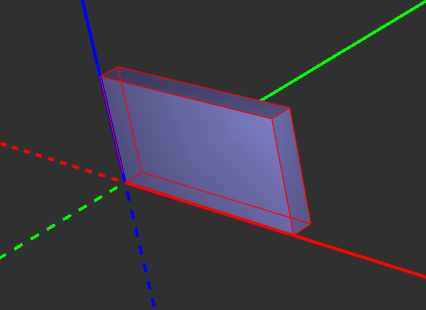
\includegraphics[height=0.7\textwidth, width=0.9\linewidth]{Figures/Thin-brick.png}
    \end{subfigure}%
    \begin{subfigure}{0.5\textwidth}
        \centering
        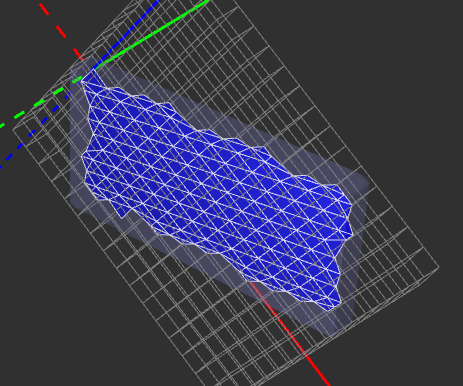
\includegraphics[height=0.7\textwidth, width=0.9\linewidth]{Figures/DC-thin-brick-mesh.png}
    \end{subfigure}
    \decoRule
    \caption{Illustration of the DC algorithm's challenges in handling objects with dimensions smaller than the cell width.}
    \label{fig:DC-analysis-thin-features}
\end{figure}

\noindent The DMC algorithm's strength in representing thin-walled structures was evident in complex datasets (Fig. \ref{fig:DC-DMC-thin-feature}), such as the rocket and room models. However, its computational intensity was a limitation in scenarios requiring real-time mesh generation.

\begin{figure}[H]
    \centering
    \begin{subfigure}{0.5\textwidth}
        \centering
        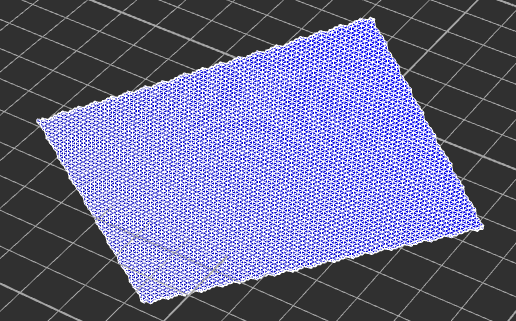
\includegraphics[height=0.7\textwidth, width=0.9\linewidth]{Figures/DC-thin-brick-new.png}
    \end{subfigure}%
    \begin{subfigure}{0.5\textwidth}
        \centering
        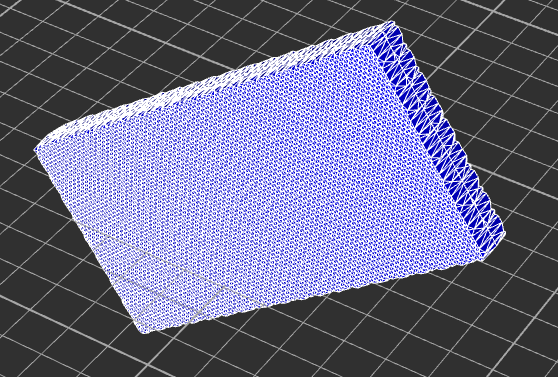
\includegraphics[height=0.7\textwidth, width=0.9\linewidth]{Figures/DMC-thin-brick.png}
    \end{subfigure}
    \decoRule
    \caption{Comparison between DC and DMC algorithms: While DC (left) struggles with thin features, DMC (right) effectively reproduces them.}
    \label{fig:DC-DMC-thin-feature}
\end{figure}

\section{Discussion}

The Dual Contouring and Dual Marching Cubes algorithms offer advanced techniques for isosurface extraction, each with strengths and limitations. The DC algorithm's ability to preserve sharp features makes it suitable for datasets where these features are crucial. However, its computational intensity and memory consumption might be limiting factors for large datasets or real-time applications. The DMC algorithm's strength lies in its ability to represent thin-walled structures. This makes it suitable for applications where the thickness or fineness of structures is a critical factor. However, its computational demand and complexity of implementation might pose challenges in specific scenarios.

In conclusion, the choice between DC and DMC depends on the application's specific requirements. For applications requiring sharp feature preservation, DC might be the preferred choice. For applications focusing on thin structures, DMC might be more suitable.